%!TEX root = ../../Master.tex
\subsubsection{CrustCrawler}
\label{subsub: CrustCrawler}

Klassen CrustCrawler er en klasse til håndtering af armens positionering. Den har til formål at fortolke det koordinat som fås fra \textbf{block} klassen, og udregne vinkelpositionerne for armens lad, således at det er muligt for armen at gribe klodsen.\\

\textbf{inverse\_kinematics}\\
Funktionen har til formål at udregne og bestemme Crustcrawlerarmens ledvinkler på baggrund af det bestemte midtpunkt for klodserne. Den tager et input (self, x, y, z, $\theta$) som beskriver et punkt for klodserne i rummet, P(x, y, z) og en vinkel for gripperen, $\theta$. Ud fra det bestemte punkt er det muligt at finde positionen til end-effektoren. x, y, z bruges til at beregne $q_1$, $q_2$, $q_3$, $q_4$. Hver q-parameter beskriver en ledvinkel for det tilsvarende led.\\

Vinklen for $q_1$ er givet ved at finde vinklen ud til punktet set fra robottens origo. Dette kan gøres ved at tage $atan2(\frac{y}{x})$ til vinklen:

\begin{equation}
q_1 = atan2(\frac{y}{x})
\end{equation}

Derefter bestemmes parametrene $r^2, s, D$. Disse er geometriske parametre som anvendes til at bestemme $q_2$ og $q_3$. Nedenfor er det illustreret i \autoref{fig:geometric_approach}, hvordan parametrene tolkes.\\

\begin{figure}[h]
\centering
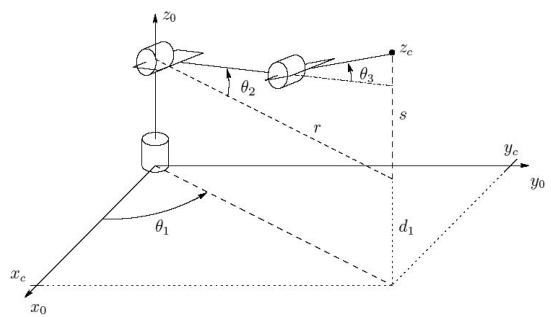
\includegraphics[scale=0.4]{images/geometric_approach}
\caption{Geometrisk bestemmelse af position.}
\label{fig:geometric_approach}
\end{figure}

$r^2$ er givet ved:

\begin{equation}
r^2 = (x - a_1 * \cos(q_1))^2 + (y - a_1 * \sin(q_1))^2
\end{equation}

Her er $a_1$ afstanden fra 1. led til 2. led, x og y er klodsens koordinat.\\

$s$ er givet ved:

\begin{equation}
s = z - d_1
\end{equation}

Her er $d_1$ højden af 2. led, z er klodsens koordinat.\\

$D$ er givet ved:

\begin{equation}
D = \frac{r^2 + s^2 - a_2^2 - d_4^2}{2 * a_2 * d_4}
\end{equation}

Her er $a_2$ afstanden mellem 2. og 3. led, $d_4$ er afstanden fra 3. led til gripperen.\\

Nu da der er blevet defineret en længde og højde til punktet, er det muligt at finde de korrekte vinkler for $q_2$ og $q_3$:

\begin{equation}
q_3 = atan2\frac{-\sqrt{1 - D^2}}{D}
\end{equation}

\begin{equation}
q_2 = atan2\frac{s}{sqrt(r^2)} - atan2\frac{d_4 * \sin(q_3)}{a_2 + d_4 * \cos(q_3)} - \frac{\pi}{2}
\end{equation}

Som sidste led i processen skal $q_4$ bestemmes. Til det er det nødvendigt at sammenligne de to $\theta$ som er blevet identificeret i \textbf{block} klassen. Da $q_4$ giver vinklen for gripperen er man interesseret i at den skal rotere mindst muligt. Altså skal det være den mindste værdi af $\theta - q_1$ som vælges:

\begin{lstlisting}[caption=if sætning $q_4$, label=q4 bestemmelse, language=Python]
        q4_1 = abs(thetas[0]) - abs(q1)
        q4_2 = abs(thetas[1]) - abs(q1)

        q4 = q4_1

        if abs(q4_2) < abs(q4_1):
            q4 = q4_2
\end{lstlisting}

\textbf{move\_to}\\
Funktionen move\_to har til formål generere den sti af punkter som armen skal følge på baggrund af de bestemte værdier i \textbf{inverse\_kinematics}. Den anvender ROS specifikke kommandoer til at bestemme motorerenes position, hastighed og udførelsestid. Dette foregår altsammen igennem JointTrajectoryPoint, som er en del af ROS robot trajectory bibliotek.\\

\begin{lstlisting}[caption=if sætning $q_4$, label=q4 bestemmelse, language=Python]
    def move_to(self, x, y, z, thetas):
        jtp = JointTrajectoryPoint(
            positions=self.inverse_kinematics(x, y, z, thetas),
            velocities=[0.5] * 4,
            time_from_start=rospy.Duration(2)
        )

        jt = JointTrajectory(
            joint_names=["joint1", "joint2", "joint3", "joint4"],
            points=[jtp]
        )

        goal = FollowJointTrajectoryGoal(trajectory=jt, goal_time_tolerance=rospy.Duration(4))

        self.client.send_goal(goal)
        self.client.wait_for_result()
\end{lstlisting}

Klassen \textbf{Crustcrawler} har ud over de ovenstående centrale funktioner, underfunktioner som specificerer bevægelsesmønstret for armen i de forskellige situationer. Såsom åbn/luk gripper, saml op/placer klods, placer klods højre/venstre og en reset position. Allesammen anvender de \textbf{move\_to} funktionen.